\chapter{High-Level Design of Ansieyes}

Having covered the theory, we now describe how Ansieyes is structured. The design had to satisfy three goals simultaneously: deliver accurate analysis for typical repositories, remain secure against adversarial inputs, and scale to large codebases without exceeding the \gls{llm}'s context limits. We addressed these through a layered architecture with clearly separated responsibilities.

\section{Architecture Overview}

Ansieyes is organised into four layers, each handling a distinct phase of the analysis pipeline. Figure \ref{fig:architecture} shows how they connect.

\begin{figure}[htb]
\centering
\begin{tikzpicture}[
    node distance=1.0cm and 0.5cm,
    layer/.style={rectangle, draw, fill=blue!8, text width=11cm, minimum height=1.2cm, align=center, rounded corners=3pt, font=\small},
    sublabel/.style={font=\scriptsize\itshape, text=gray},
    arrow/.style={-{Stealth[length=2.5mm]}, thick}
]
\node[layer] (trigger) {\textbf{Trigger Layer}\\GitHub Actions Workflows --- Issue Opened / Labelled / PR Merged};
\node[layer, below=of trigger] (security) {\textbf{Security and Preprocessing Layer}\\Prompt Injection Detection $\bullet$ Input Sanitisation $\bullet$ Duplicate Detection};
\node[layer, below=of security] (analysis) {\textbf{Analysis Engine Layer}\\GeminiIssueAnalyser (Surgeon) $\bullet$ LibrarianAnalyser (Pass 1) $\bullet$ PRAnalyser};
\node[layer, below=of analysis] (data) {\textbf{Data Models and Utilities}\\Pydantic Models $\bullet$ Configuration $\bullet$ Output Formatting};

\draw[arrow] (trigger) -- (security);
\draw[arrow] (security) -- (analysis);
\draw[arrow] (analysis) -- (data);
\end{tikzpicture}
\caption[Layered architecture of Ansieyes]{\textbf{Layered architecture of Ansieyes}}
\vspace{2mm}
\label{fig:architecture}
\end{figure}

Figure \ref{fig:dfd0} presents the DFD-0 context diagram of Ansieyes, showing how the system interacts with external entities such as GitHub, the developer, the Gemini AI model, the target repository, and the security modules.

\begin{figure}[htb]
\centering
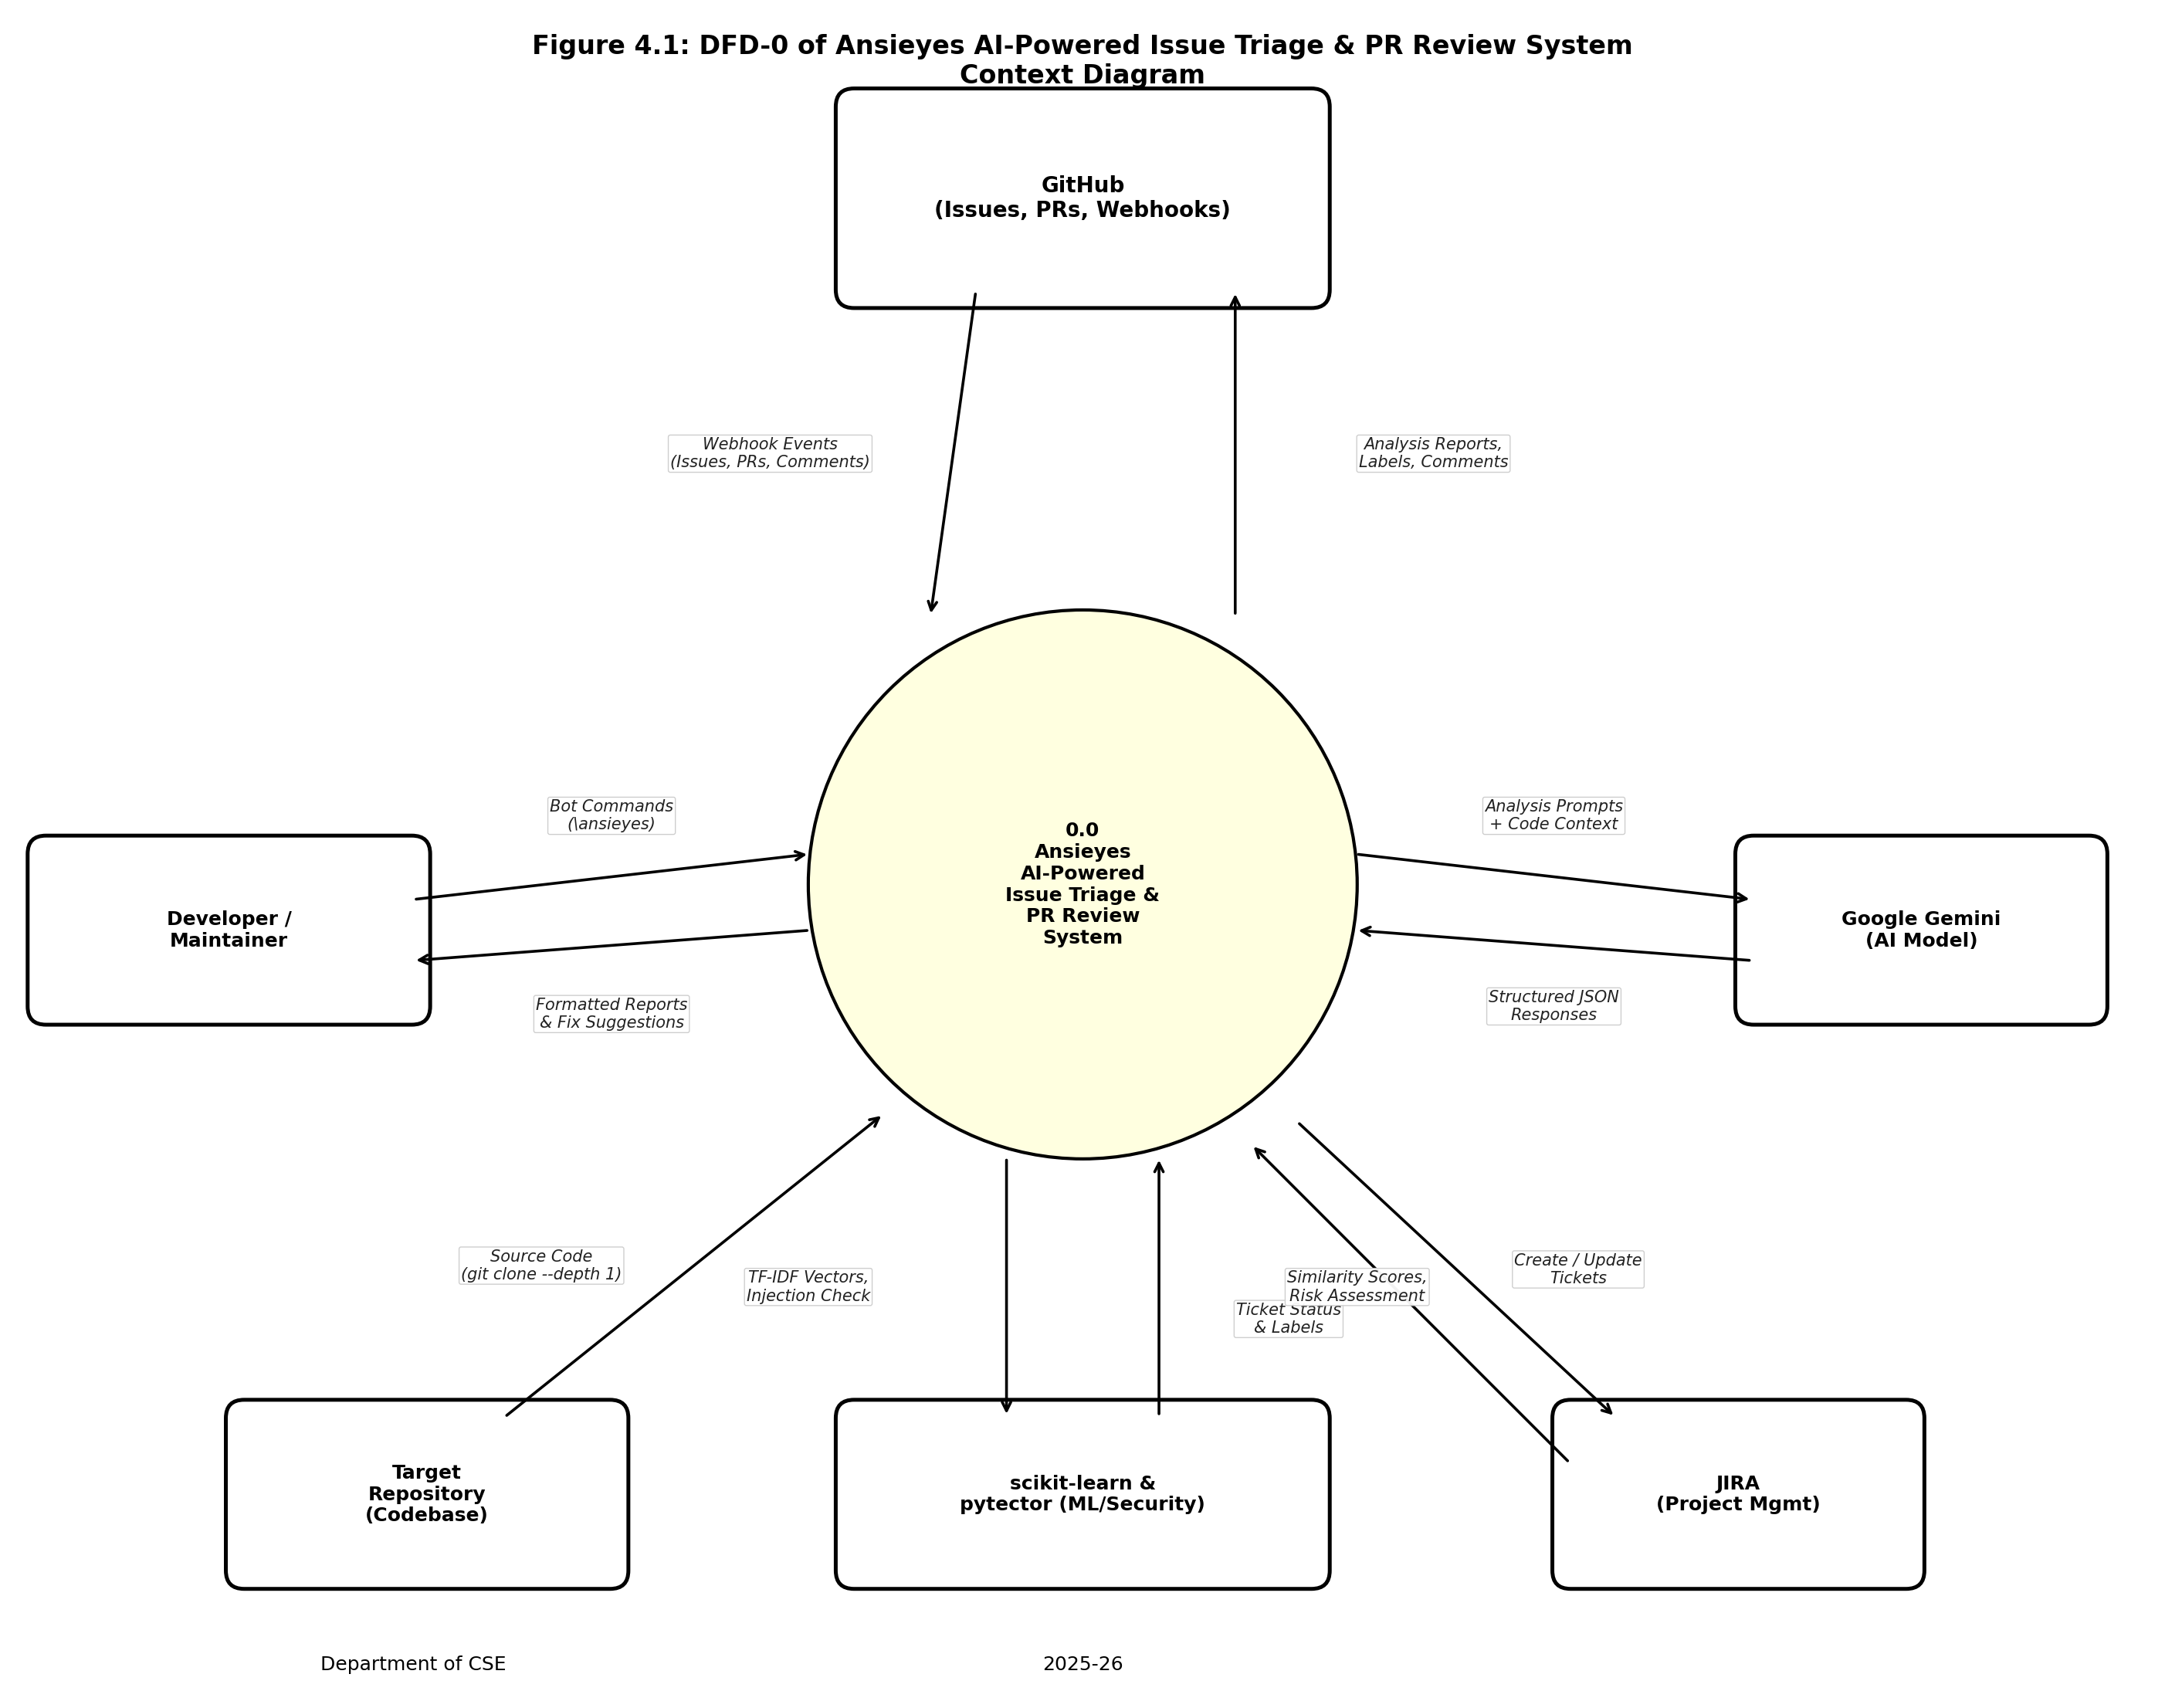
\includegraphics[width=1.0\textwidth]{Figures/report_image_1}
\caption[DFD-0 of Ansieyes AI-Powered Issue Triage and PR Review System Context Diagram]{\textbf{DFD-0 of Ansieyes AI-Powered Issue Triage and PR Review System Context Diagram}}
\vspace{2mm}
\label{fig:dfd0}
\end{figure}

Figure \ref{fig:dfd1} decomposes the system further into its internal processes: the Webhook Handler, Prompt Injection Detector, Duplicate Detector, Issue Triager (Librarian + Surgeon), PR Reviewer, Auto-Fixer, and Output Formatter.

\begin{figure}[htb]
\centering
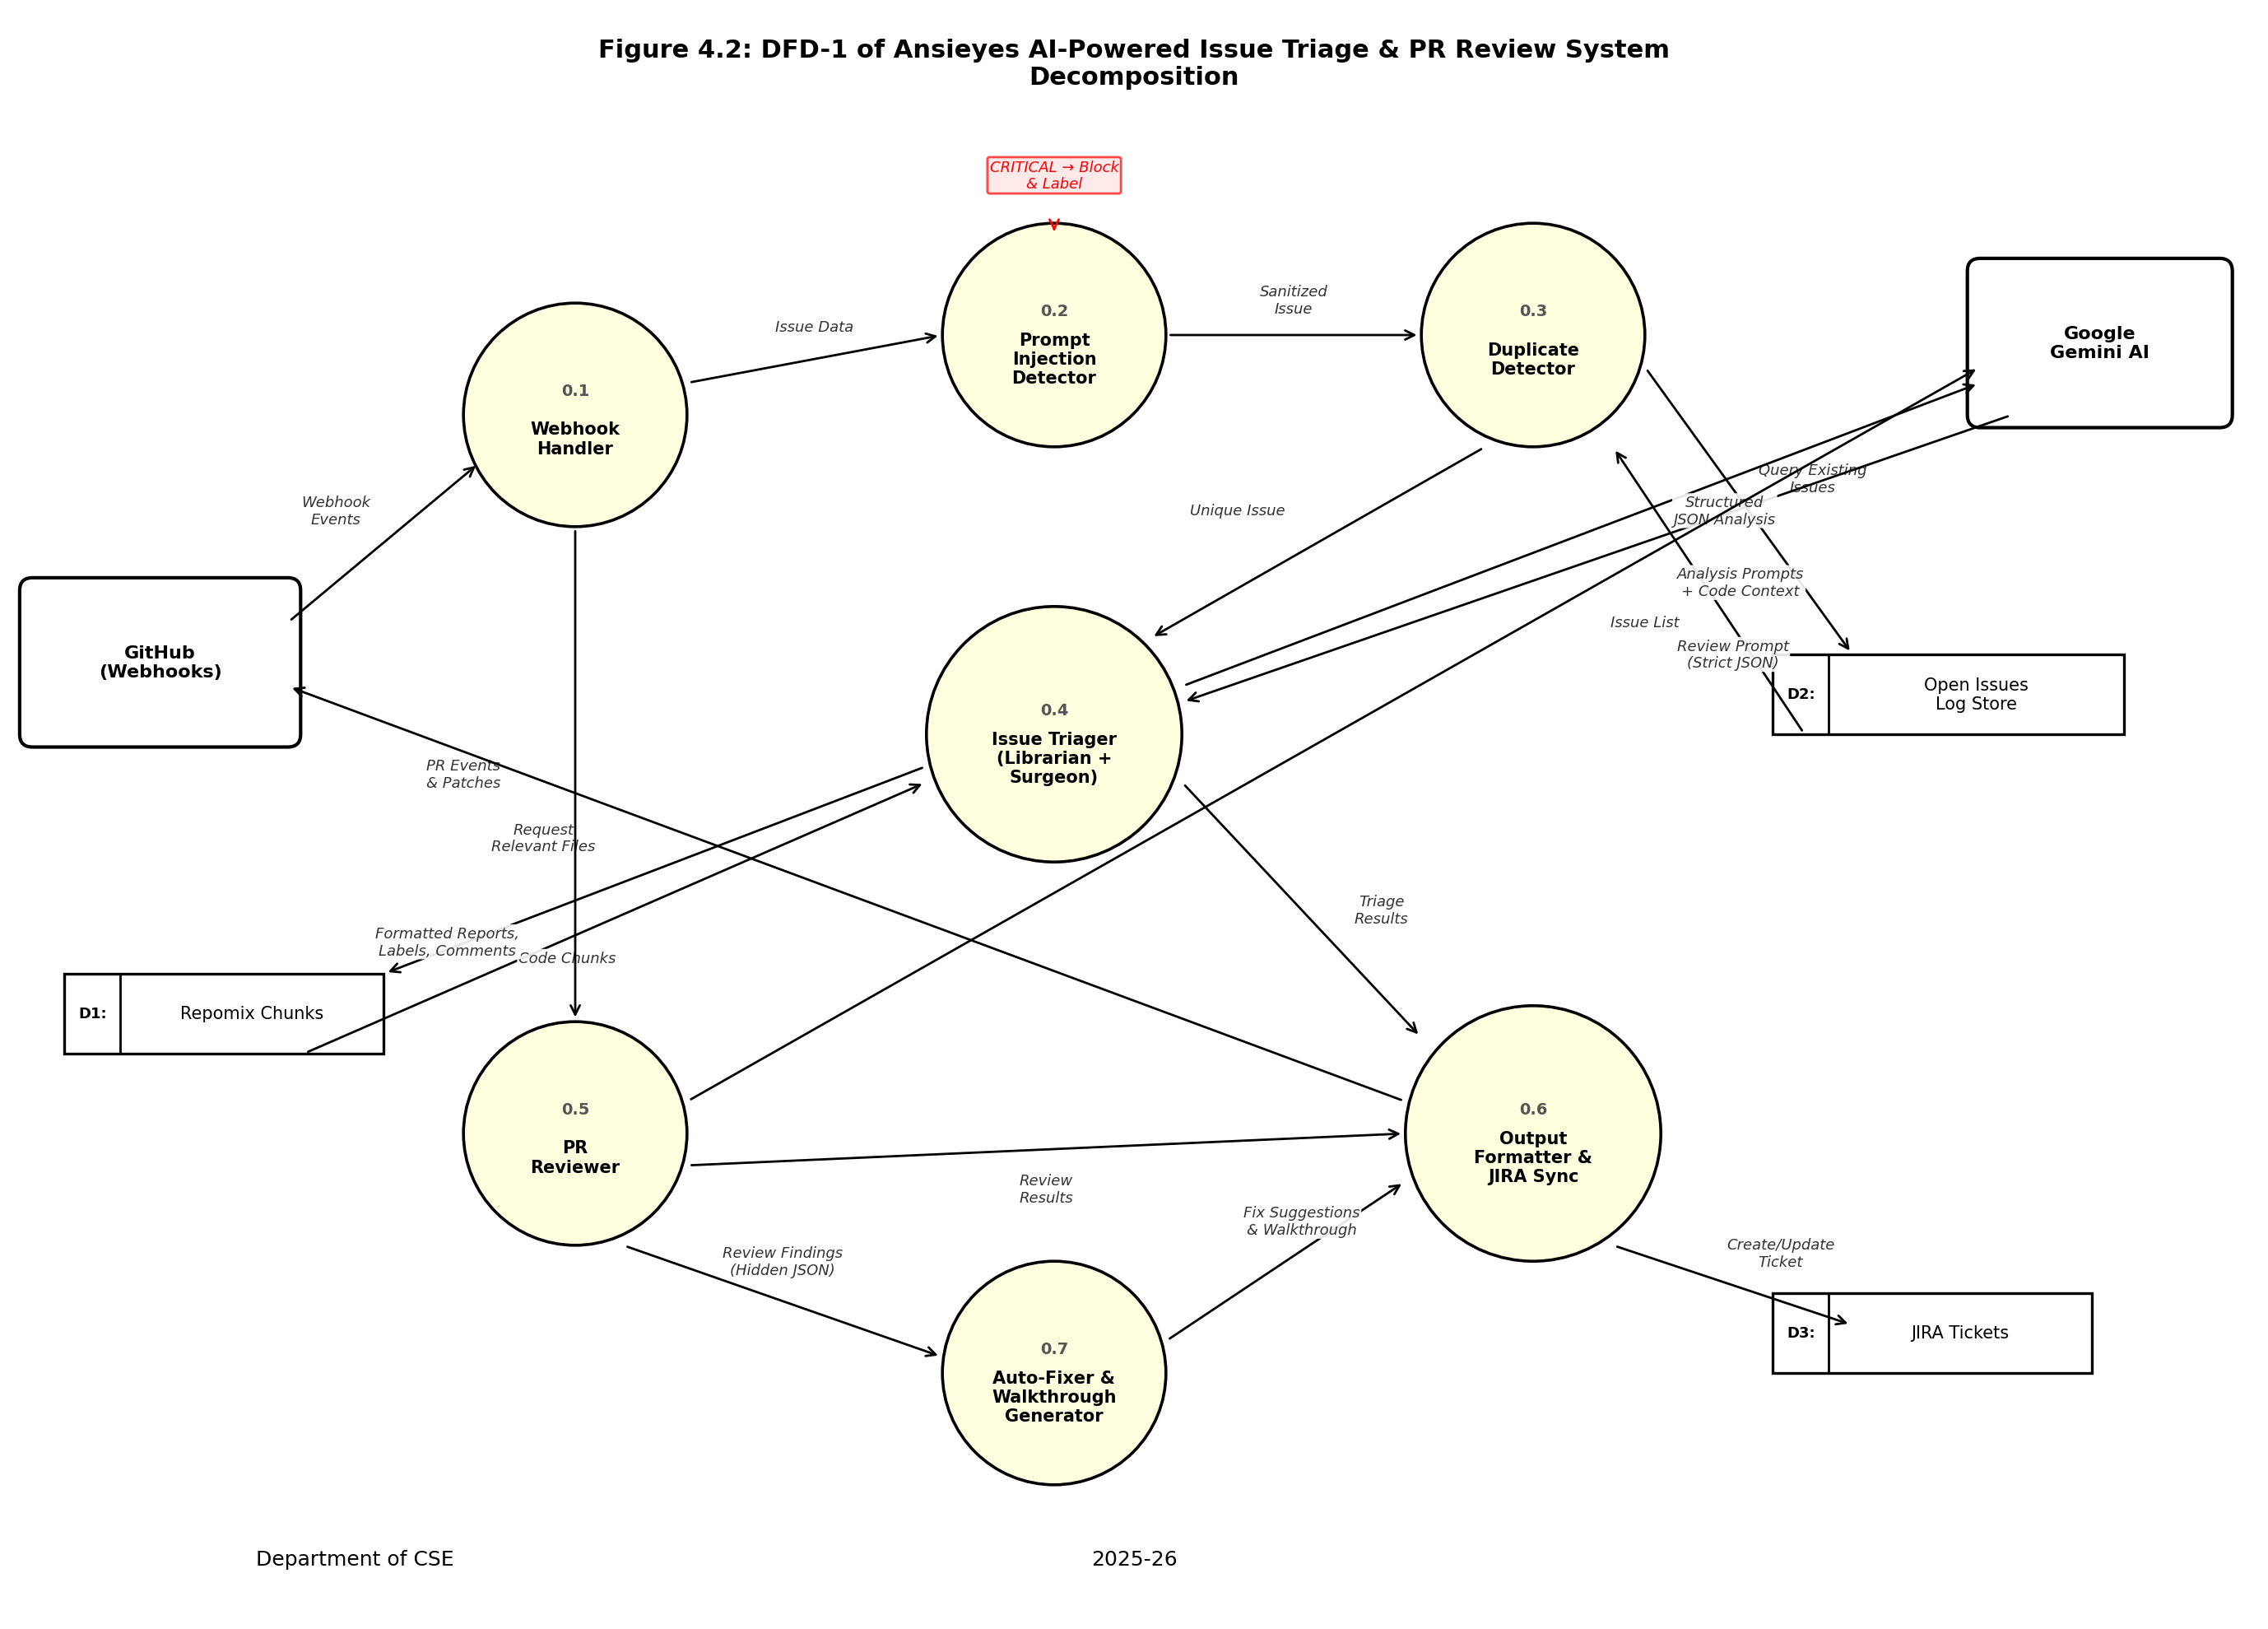
\includegraphics[width=1.0\textwidth]{Figures/report_image_2}
\caption[DFD-1 of Ansieyes AI-Powered Issue Triage and PR Review System Decomposition]{\textbf{DFD-1 of Ansieyes AI-Powered Issue Triage and PR Review System Decomposition}}
\vspace{2mm}
\label{fig:dfd1}
\end{figure}

\subsection{Trigger Layer}
The entry point is a set of GitHub Actions workflows that listen for repository events. When a new issue is created, a workflow fires and kicks off the analysis pipeline. We provide six workflow configurations to suit different team preferences:

\begin{itemize}
\item Analyse every new issue automatically.
\item Analyse only issues with a specific label (to control \gls{api} costs).
\item Bulk re-analyse all open issues after a \gls{pr} merge (so analyses reflect the latest code).
\item Label-filtered bulk analysis.
\item Two-pass analysis using the Librarian--Surgeon pipeline.
\item \gls{pr} review on labelled pull requests.
\end{itemize}

\subsection{Security and Preprocessing Layer}
Every issue passes through this layer before reaching the analyser. It performs three checks: prompt injection detection (described in detail below), input sanitisation to mask any \gls{api} keys or credentials accidentally included in the issue text, and duplicate detection to avoid wasting \gls{api} calls on already-reported problems.

\subsection{Analysis Engine Layer}
Three specialised analysers live in this layer. The GeminiIssueAnalyser (which we call the Surgeon) handles deep issue analysis. The LibrarianAnalyser handles file selection for the two-pass mode. The PRAnalyser provides pull request review with repository-type-specific prompts.

\subsection{Data Models Layer}
All analysis outputs are defined as Pydantic models, which enforce type safety and value constraints at runtime. If the \gls{llm} produces a confidence score outside the 0--1 range, for example, Pydantic catches it before the result reaches the user.

\subsection{Configuration Management}
Rather than hardcoding parameters throughout the codebase, Ansieyes centralises its configuration into two files. The first, \texttt{triage.config.json}, controls the analysis pipeline---it specifies the Gemini model to use, the similarity threshold for duplicate detection, the maximum file count for single-pass mode, and feature flags for enabling or disabling specific modules. The second, \texttt{pr\_prompt\_config.yml}, maps repository URL patterns to specialised \gls{pr} review prompts so that a Python project gets different review criteria than, say, a JavaScript frontend. This separation means that teams can tune Ansieyes for their specific workflow without touching any source code; they simply edit the relevant configuration file and the changes take effect on the next run.

\subsection{Workflow Orchestration}
The six GitHub Actions workflows described in the Trigger Layer do not operate in isolation---they form a coordinated pipeline. The issue analysis workflow triggers first and posts its results as a comment; if duplicate detection is enabled, the duplicate detection workflow runs in parallel and adds a separate label and comment. The bulk re-analysis workflow listens for \gls{pr} merge events and re-triggers analysis on all open issues so that triage results stay current with the latest code. The \gls{pr} review workflow operates on its own event stream. Coordination between these workflows is handled through GitHub's native event system and shared labels, which means no external orchestration service is needed. This design keeps the deployment simple---repository owners just copy the workflow files into their \texttt{.github/workflows} directory and set the required secrets.

\section{Data Model Design}

We defined five core models to represent the system's outputs. Table \ref{tab:models} summarises their key fields.

\begin{table}[htb]
\centering
\renewcommand{\arraystretch}{1.3}
\setlength{\arrayrulewidth}{0.5mm}
\fontsize{10}{12}\selectfont
\caption[Core data models and their fields]{\textbf{Core data models and their fields}}
\vspace{2mm}
\label{tab:models}
\begin{tabular}{|p{3.8cm}|p{8cm}|}
\hline
\textbf{Model} & \textbf{Key Fields} \\
\hline
IssueAnalysis & issue\_type, severity, root\_cause\_analysis, proposed\_solutions, confidence\_score, analysis\_summary \\
\hline
RootCauseAnalysis & primary\_cause, contributing\_factors, affected\_components, related\_code\_locations \\
\hline
CodeSolution & description, code\_changes, location (file, line, function, class), rationale \\
\hline
DuplicateDetectionResult & is\_duplicate, duplicate\_of, similarity\_score, similarity\_reasons, recommendation \\
\hline
InjectionResult & is\_injection, risk\_level, confidence\_score, detected\_patterns, sanitized\_text \\
\hline
\end{tabular}
\end{table}

The IssueAnalysis model deserves a closer look. Its \texttt{issue\_type} field accepts one of three values: bug, enhancement, or feature\_request. The \texttt{severity} field ranges from low to critical. The \texttt{root\_cause\_analysis} is itself a nested object containing the primary cause as text, a list of contributing factors, a list of affected components, and a list of code locations (each with file path, line number, function name, and class name). Proposed solutions follow a similar structure, with each solution specifying where in the code the change should be made and why.

\section{Two-Pass Librarian--Surgeon Architecture}

For small to medium repositories, loading the entire codebase into a single Gemini prompt works well. But enterprise-scale projects can have hundreds of thousands of lines of code, far more than the model can process at once. Even for projects that technically fit, stuffing irrelevant code into the context dilutes the model's attention and wastes tokens.

Our solution splits the analysis into two passes, as shown in Figure \ref{fig:twopass}.

\begin{figure}[htb]
\centering
\begin{tikzpicture}[
    node distance=0.8cm,
    block/.style={rectangle, draw, fill=blue!8, text width=5cm, minimum height=1cm, align=center, rounded corners=2pt, font=\small},
    data/.style={rectangle, draw, fill=orange!10, text width=5cm, minimum height=0.8cm, align=center, rounded corners=2pt, font=\small\itshape},
    arrow/.style={-{Stealth[length=2.5mm]}, thick}
]
\node[data] (input) {Issue Title + Description};
\node[block, below=of input] (lib) {\textbf{Pass 1: Librarian}\\Analyse directory chunks};
\node[data, below=of lib] (files) {List of Relevant Files};
\node[block, below=of files] (repomix) {Generate Targeted Repomix};
\node[data, below=of repomix] (context) {Focused Codebase Context};
\node[block, below=of context] (surgeon) {\textbf{Pass 2: Surgeon}\\Deep issue analysis};
\node[data, below=of surgeon] (output) {Structured Analysis Output};

\draw[arrow] (input) -- (lib);
\draw[arrow] (lib) -- (files);
\draw[arrow] (files) -- (repomix);
\draw[arrow] (repomix) -- (context);
\draw[arrow] (context) -- (surgeon);
\draw[arrow] (surgeon) -- (output);
\end{tikzpicture}
\caption[Two-pass Librarian--Surgeon flow]{\textbf{Two-pass Librarian--Surgeon flow}}
\vspace{2mm}
\label{fig:twopass}
\end{figure}

\subsection{Pass 1: The Librarian}
The Librarian receives the issue description along with a set of directory-level ``chunks''---compressed summaries of each top-level directory in the repository. For each chunk, it asks Gemini: \textit{which files in this directory are relevant to the reported issue?} The model returns a list of file paths, which the Librarian validates (discarding paths that lack a file extension, exceed 200 characters, or start with comment markers). A dependency analysis step can optionally include files imported by the initially identified set.

\subsection{Pass 2: The Surgeon}
A new Repomix output is generated containing only the files the Librarian identified. The Surgeon---which is just the standard GeminiIssueAnalyser---runs its full analysis against this focused context. Because it is working with a fraction of the original codebase, the analysis is both cheaper and more precise.

\subsection{Token Savings}
If a repository has $N$ files in total and the Librarian selects $R$ of them, the token reduction is approximately $1 - R/N$. In practice, we observed reductions between 57\% and 70\% on medium to large repositories. For very large codebases that exceed the single-pass context limit entirely, the two-pass approach is the only option.

\section{Security Architecture}

We designed the security module as three independent detectors whose outputs are aggregated. Figure \ref{fig:security} illustrates the pipeline.

\begin{figure}[htb]
\centering
\begin{tikzpicture}[
    node distance=0.6cm and 1.5cm,
    block/.style={rectangle, draw, fill=blue!8, text width=3.2cm, minimum height=1cm, align=center, rounded corners=2pt, font=\small},
    input/.style={rectangle, draw, fill=orange!10, text width=3.5cm, minimum height=0.8cm, align=center, rounded corners=2pt, font=\small\itshape},
    output/.style={rectangle, draw, fill=green!10, text width=3.5cm, minimum height=0.8cm, align=center, rounded corners=2pt, font=\small},
    arrow/.style={-{Stealth[length=2.5mm]}, thick}
]
\node[input] (input) {Issue Description};
\node[block, below left=1cm and 0.3cm of input] (ml) {ML-Based\\Detector};
\node[block, below=1cm of input] (pattern) {Pattern\\Matching};
\node[block, below right=1cm and 0.3cm of input] (heuristic) {Heuristic\\Analysis};
\node[block, below=2.8cm of input] (agg) {Risk Aggregation};
\node[output, below=of agg] (result) {Risk Level + Confidence};

\draw[arrow] (input) -- (ml);
\draw[arrow] (input) -- (pattern);
\draw[arrow] (input) -- (heuristic);
\draw[arrow] (ml) -- (agg);
\draw[arrow] (pattern) -- (agg);
\draw[arrow] (heuristic) -- (agg);
\draw[arrow] (agg) -- (result);
\end{tikzpicture}
\caption[Multi-layered prompt injection detection pipeline]{\textbf{Multi-layered prompt injection detection pipeline}}
\vspace{2mm}
\label{fig:security}
\end{figure}

The aggregator takes the highest risk level reported by any individual detector. This conservative strategy means that even if an attacker manages to slip past one layer, the others can still catch the attempt. Risk levels range from Safe through Low, Medium, and High to Critical. Issues flagged as High or Critical are blocked from analysis entirely; Low and Medium risks proceed with a warning.

\section{Duplicate Detection Design}

We offer two approaches, each with its own trade-offs.

The \textbf{Gemini-based} detector sends the new issue along with all existing open issues to the model and asks it to evaluate semantic similarity. It can catch duplicates even when the wording is completely different---for example, one issue saying ``the app crashes on login'' and another saying ``authentication module throws a null pointer exception.'' The downside is that each check costs an \gls{api} call.

The \textbf{cosine similarity} detector works offline. It preprocesses issue text (lowercasing, removing special characters), builds \gls{tfidf} vectors with unigram and bigram features, and computes cosine similarity. We weight the title 2x relative to the description, since titles tend to carry the most distinctive information. Issues above a 0.6 similarity threshold are flagged. This method is fast (under 100 milliseconds) but misses semantic duplicates that use different words.

\section{PR Review Design}

The pull request reviewer extends Ansieyes to code review. It uses a \gls{yaml} configuration file that maps repository URL patterns (for example, repositories with ``python'' in the name) to specialised review prompts. The reviewer analyses the \gls{pr} diff, generates file-specific comments with line numbers, and produces an overall assessment broken into strengths, issues, and suggestions.

The design choices described in this chapter were shaped by practical constraints: \gls{api} costs, context window limits, and the need to handle adversarial inputs. The next chapter explains how we turned these designs into working code.

\section{Summary}

This chapter described the high-level design of Ansieyes, covering its four-layer architecture, data model design, the two-pass Librarian--Surgeon strategy for scaling to large codebases, the multi-layered security pipeline for prompt injection defence, the dual duplicate detection approach, and the PR review subsystem. These design decisions translate the theoretical foundations from the previous chapter into a concrete system structure that the next chapter implements.
